\chapter[Memes]{Memes}
\label{sec:fullmemes}
\section{Dufu is very busy}


\zh{杜甫很忙}

Le poète chinois Du Fu de la dynastie Tang a également connu un retour fulgurant sous la forme de peintures détournées le mettant en scène dans des situations improbables : ``Du Fu est vraiment très occupé'' \zh{杜甫很忙}. 


Du Fu is Busy is a photoshop meme based on a drawing of the Tang Dynasty Chinese poet Du Fu (\zh{杜甫}). The images are typically edited by putting the poet in odd situations and giving him new clothes, accessories and hairstlyes.

\url{http://knowyourmeme.com/memes/du-fu-is-busy}
\url{http://wenku.baidu.com/view/941e25c805087632311212aa.html}

\begin{figure}[ht]
    \centering
    \subfloat[]{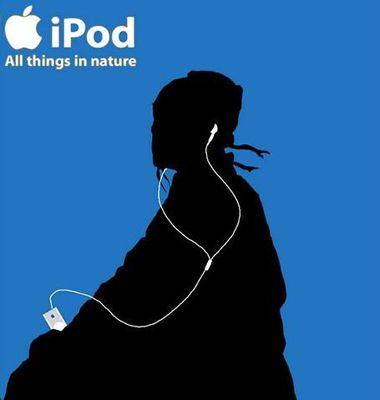
\includegraphics[scale=.4]{figures/annexes/dufu/8c7.jpg}}
    \subfloat[]{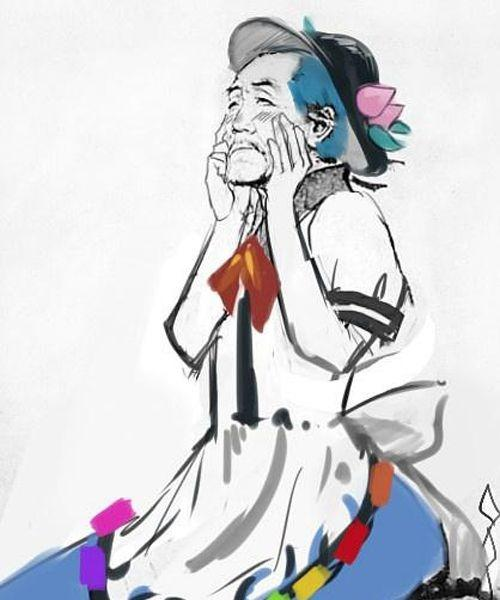
\includegraphics[scale=.3]{figures/annexes/dufu/8dd.jpg}}
    \subfloat[]{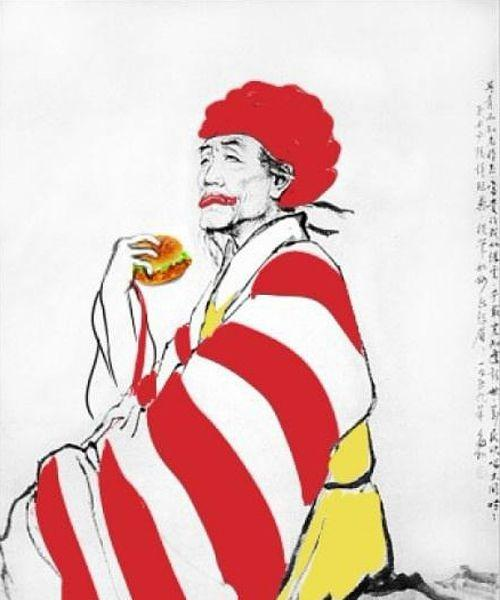
\includegraphics[scale=.3]{figures/annexes/dufu/b5f.jpg}}
    \newline
    \subfloat[]{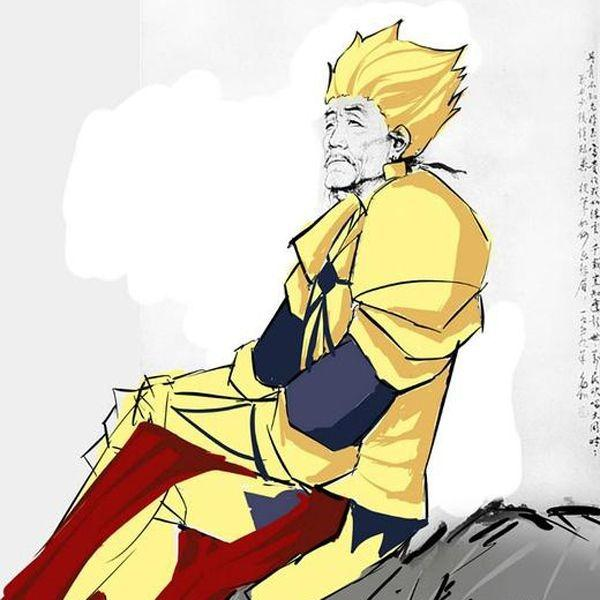
\includegraphics[scale=.3]{figures/annexes/dufu/bb3.jpg}}
    \subfloat[]{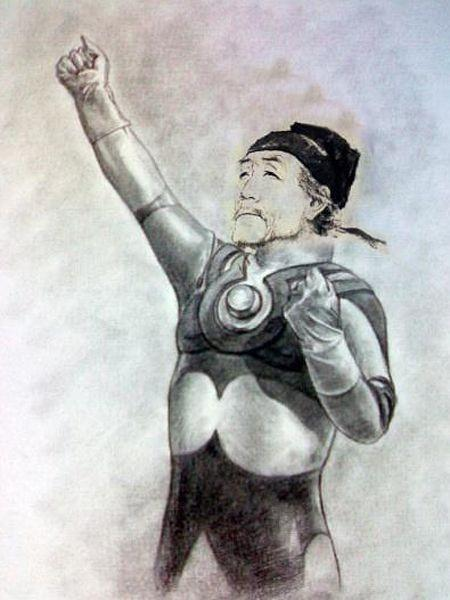
\includegraphics[scale=.3]{figures/annexes/dufu/bd8.jpg}}
    \subfloat[]{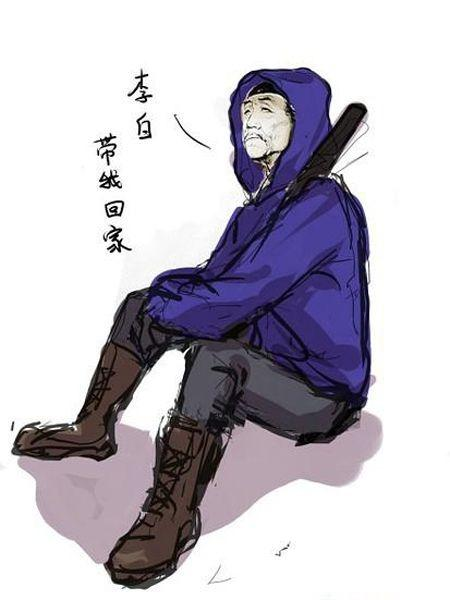
\includegraphics[scale=.3]{figures/annexes/dufu/d09.jpg}}
    \caption{
      Dufu is very busy 
    }
\end{figure}

\clearpage

\section{Yuan Fang, qu'en penses tu?}

Une série policière très prisée présentant un couple de détectives enquêtant dans la Chine médiévale procura notamment de bonne doses de rire aux spectateurs. Dialogue récurrent de la série, la phrase ``Yuanfang, qu'en penses-tu'' (\zh{元芳,你怎么看?}) s'est hissé en peu de temps à une célébrité semblable au \textit{``élémentaire''} de Sherlock Holmes au Dr. Watson. 


\begin{figure}[ht]
    \centering
    \subfloat[]{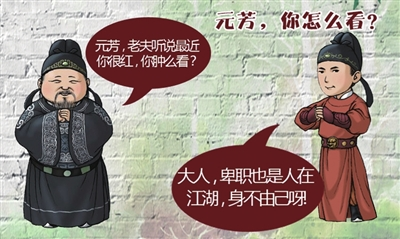
\includegraphics[scale=.4]{figures/annexes/yuanfang/50fa21e4d4994.jpg}}
    \subfloat[]{
\includegraphics[scale=.3]{figures/annexes/yuanfang/960a304e251f95ca67b3a568c9177f3e660952ad.jpg}}
    \subfloat[]{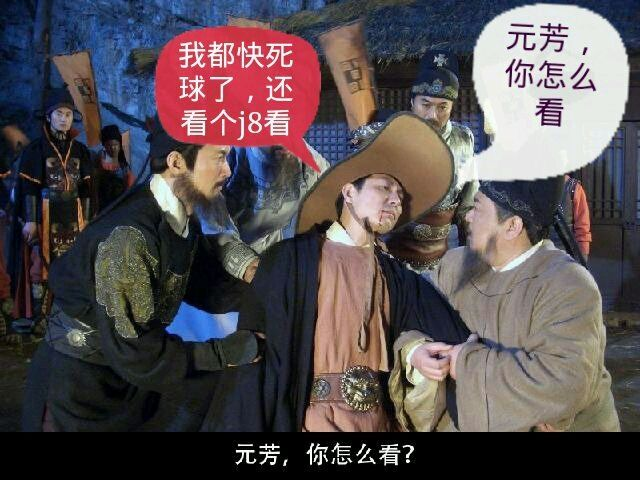
\includegraphics[scale=.3]{figures/annexes/yuanfang/2012102210340971752.jpg}}
    \newline
    \subfloat[]{
\includegraphics[scale=.3]{figures/annexes/yuanfang/d4f21080968f3187.png}}
    \subfloat[]{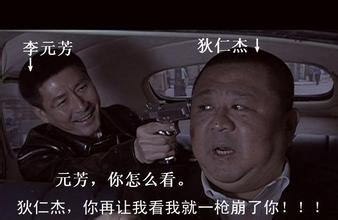
\includegraphics[scale=.3]{figures/annexes/yuanfang/u=4077910649,4163896412&fm=21&gp=0.jpg}}
    \subfloat[]{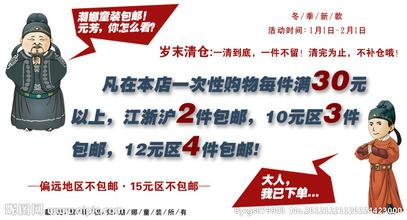
\includegraphics[scale=.3]{figures/annexes/yuanfang/ad.jpg}}
    \caption{
      Dufu is very busy 
    }
\end{figure}

\clearpage

\section{Biaoge}



\begin{figure}[ht]
    \centering
    \subfloat[]{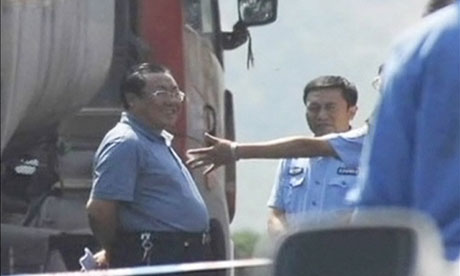
\includegraphics[scale=.4]{figures/annexes/biaoge/Yang-Dacai-smiling.jpg}}
    \subfloat[]{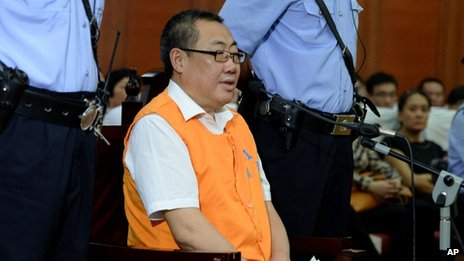
\includegraphics[scale=.6]{figures/annexes/biaoge/biaoge-jailed.jpg}}
    \caption{      
            \textit{``Yang Dacai, dubbed Brother Wristwatch, shown smiling at the scene of a crash in the photo that first gained him notoriety on social media. Photograph: Reuters/CCTV''}, d'après le Guardian \url{http://www.theguardian.com/world/2013/sep/05/china-brother-wristwatch-yang-dacai-sentenced}, consulté le 7 Juillet 2014 à 12:11.\textit{``Yang pleaded guilty to corruption charges last week''}, d'après la BBC \url{http://www.bbc.com/news/world-asia-china-23956170}, consulté le 7 Juillet 2014 à 12:11.
    }
\end{figure}

\begin{figure}[h!]
    \centering
    \subfloat[]{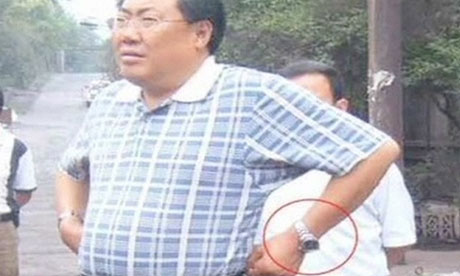
\includegraphics[scale=.4]{figures/annexes/biaoge/Yang-Dacai-wearing-one-of-010.jpg}}
    \subfloat[]{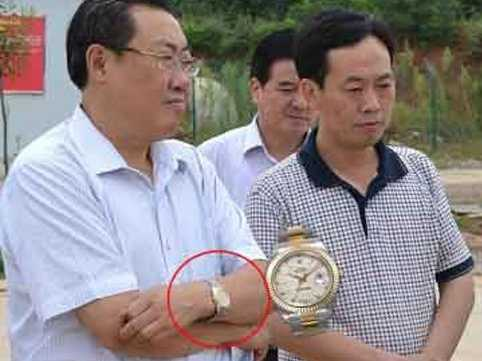
\includegraphics[scale=.3]{figures/annexes/biaoge/chinese-official-photographed-smirking-after-a-traffic-accident-that-left-36-dead-has-been-fired.jpg}}
    \newline
    \subfloat[]{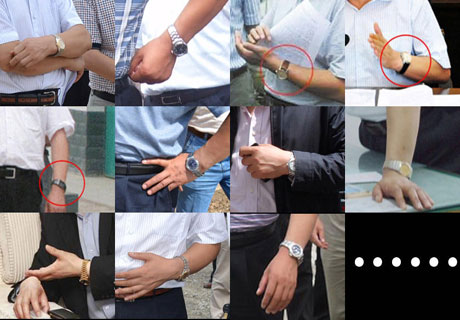
\includegraphics[scale=.3]{figures/annexes/biaoge/201209120198.jpg}}
    \subfloat[]{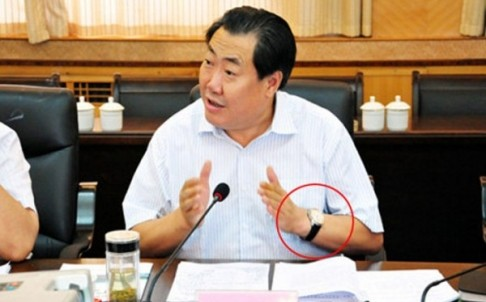
\includegraphics[scale=.3]{figures/annexes/biaoge/yang-dacai.jpg}}
    \caption{
      Dufu is very busy 
    }
\end{figure}

\clearpage
\section{Sex Tape }

\url{http://en.wikipedia.org/wiki/Lei_Zhengfu}

\url{http://www.viddler.com/v/41bf67b2}, consulté le 7 Juillet à 12:32

``Sex tape official stands trial in Chongqing'' d'après le \textit{People's Daily}, \url{http://english.peopledaily.com.cn/90882/8290628.html}, consulté le 7 Juillet à 12:32

http://www.dailymail.co.uk/news/article-2239300/Zhao-Hongxia-Teenage-honeytrap-brought-Chinese-Communist-Party-official-sex-tape-pictures-leaked-online.html

\clearpage
\section{Qiegao}

http://world.time.com/2012/12/05/dont-let-them-eat-cake-how-ethnic-tensions-in-china-explode-on-the-streets/


\begin{figure}[h!]
    \centering
    \subfloat[Un vendeur de qiegao]{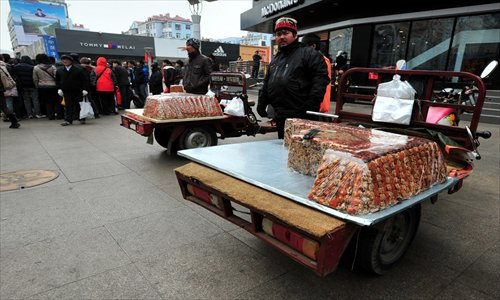
\includegraphics[scale=.65]{figures/annexes/qiegao/91914349-4fce-4373-b7dc-9fe05a0a28bf.jpeg}}
    \subfloat[Le gâteau]{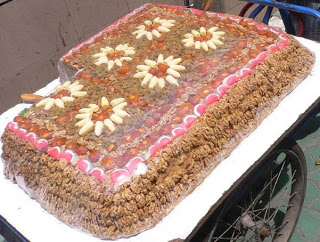
\includegraphics[scale=.7]{figures/annexes/qiegao/Qie-Gao.jpeg}}
    \newline
    \subfloat[Une image de l'affrontement avec la police posté par un utilisateur de Sina Weibo]{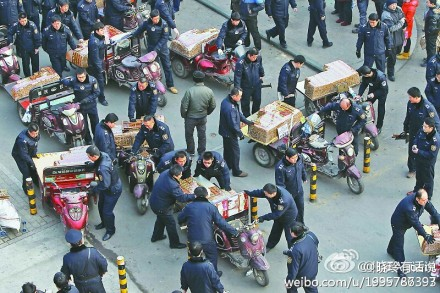
\includegraphics[scale=.65]{figures/annexes/qiegao/1.jpg}}
    \subfloat[Création d'un internaute montrant combien le qiegao est cher]{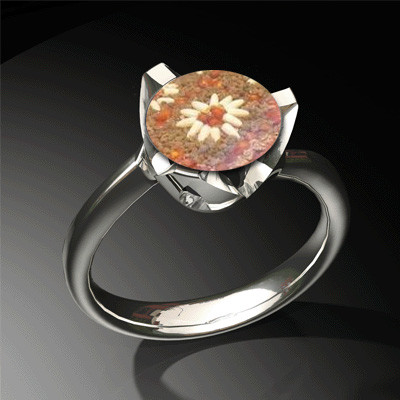
\includegraphics[scale=.66]{figures/annexes/qiegao/2.jpg}}
    \caption{
      Qiegao
    }
\end{figure}

\clearpage
\section{The Voice of China}

\url{http://en.wikipedia.org/wiki/The_Voice_of_China}

\begin{figure}[h!]
    \centering
    \subfloat[Logo Officiel de The Voice of China]{
\includegraphics[scale=.47]{figures/annexes/thevoice/The_Voice_of_China_-_official_logo.jpg}}
    \subfloat[Les membres du Jury de l'édition 2014]{
\includegraphics[scale=.5]{figures/annexes/thevoice/The_Voice_of_China_S2.jpg}}
    \newline
    \subfloat[``The Voice devient le sujet le plus discuté du mois de Juillet'', d'après Hi News, \url{http://www.hinews.cn/news/system/2012/08/25/014863154.shtml}, consulté le 7 Juillet à 14:32]{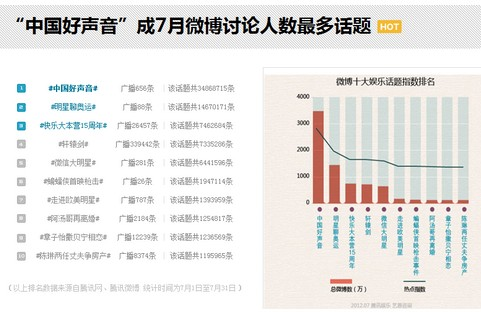
\includegraphics[scale=.8]{figures/annexes/thevoice/weibo-trends.jpg}}
    \subfloat[Un dessin posté par un utilisateur de Sina Weibo]{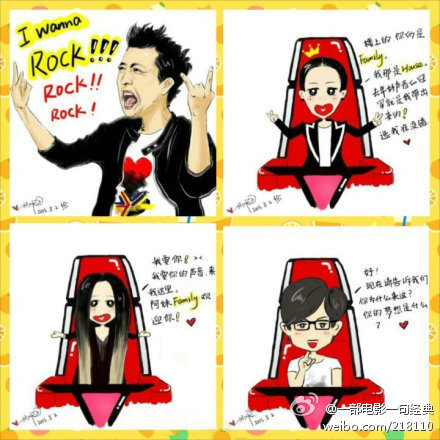
\includegraphics[scale=.42]{figures/annexes/thevoice/7ff5fbaftw1e7ilgxti2bj20c80c8gn2.jpg}}
    \caption{
      The Voice of China : Illustrations
    }
\end{figure}


\clearpage
\section{Moyan}

\url{http://en.wikipedia.org/wiki/Mo_Yan}

% \begin{figure}[h!]
%     \centering
%     \subfloat[Logo Officiel de The Voice of China]{
\includegraphics[scale=.47]{figures/annexes/thevoice/The_Voice_of_China_-_official_logo.jpg}}
%     \subfloat[Les membres du Jury de l'édition 2014]{
\includegraphics[scale=.5]{figures/annexes/thevoice/The_Voice_of_China_S2.jpg}}
%     \newline
%     \subfloat[``The Voice devient le sujet le plus discuté du mois de Juillet'', d'après Hi News, \url{http://www.hinews.cn/news/system/2012/08/25/014863154.shtml}, consulté le 7 Juillet à 14:32]{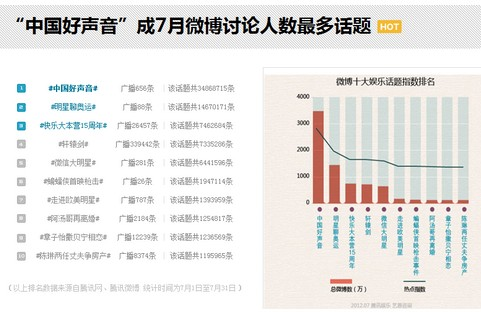
\includegraphics[scale=.8]{figures/annexes/thevoice/weibo-trends.jpg}}
%     \subfloat[Un dessin posté par un utilisateur de Sina Weibo]{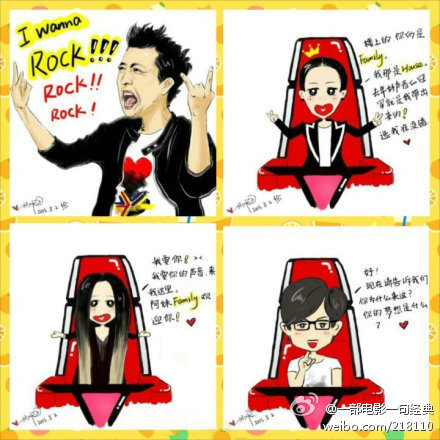
\includegraphics[scale=.42]{figures/annexes/thevoice/7ff5fbaftw1e7ilgxti2bj20c80c8gn2.jpg}}
%     \caption{
%       The Voice of China : Illustrations
%     }
% \end{figure}
